\documentclass[border=5mm, tikz]{standalone}

\usepackage{tikz}

\usetikzlibrary{positioning, arrows.meta, automata}

% Document
\begin{document}

    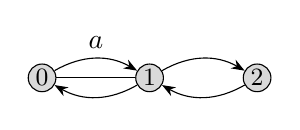
\begin{tikzpicture}[circ/.style={circle,
    draw=black, % Circle colour (edge).
    fill=gray, % Circle fill colour.
    fill opacity=0.3,
    text opacity=1,
    inner sep=0pt,
    minimum size=10pt,
    font=\small},
    arrow/.style={-Stealth}]

        % Nodes.
        \node[circ] (0) {0};
        \node[circ, right = of 0] (1) {1};
        \node[circ, right = of 1] (2) {2};

        % Undirected edges.
        \foreach \i/\j in {0/1}
        \draw (\i) -- (\j);

        % Directed edges.
        \foreach \i/\j in {1/0, 1/2, 2/1}
        \draw[arrow] (\i) to[bend left] (\j);

        % Labeled directed edges.
        \foreach \i/\j/\txt/\p in {0/1/$a$/above}
        \draw[arrow] (\i) to[bend left] node[draw=none, \p] {\txt} (\j);
    \end{tikzpicture}

\end{document}